% questions.tex —— 1977 年·青海卷 · 题目内容片段（无答案）
% 由 tools/generate_projects.py 依来源总账自 1977/1977_数学真题_青海_试题.md 生成，勿手改（改源 MD 后重跑）


\gkpart{数学试题解}

\begin{gktip}
\textbf{来源说明}：本题面依据固定源 PDF《青海1977年高考数学试题解》第 1—4 页逐题转录。固定源是题面与解答连续出现的扫描材料（书籍页码 122—124，第 4 页扫描不完整、无页码可见），而不是无答案试卷；正式题为第一至第十题，末尾“参考题”两题不计入题量。原卷未标分值、不分文理、无附加题。原卷第四题的两个子项编号为“1．”“2．”，本库按小问格式重排为（1）（2），未增删题干内容。
\end{gktip}

\par\medskip

\begin{question}
\gkti{1}计算：

\nopagebreak[4]
\[
\frac{a}{a-b}-\frac{b}{a+b}+\frac{2ab}{a^2-b^2}\cdot(a\ne\pm b).
\]

\Needspace{0.4\textheight}
\end{question}
\begin{question}
\gkti{2}如图，$AB$ 是 $\odot O$ 的直径，$AC$ 是 $\odot O$ 的切线，连接 $BC$ 与 $\odot O$ 相交于 $D$ 点，而且 $\angle ABC=45^\circ$。求证 $BD=DC$。

\begin{gktip}
原源 PDF 第 1 页附有圆、切线与弦的示意图；LaTeX 版按源图重绘。
\end{gktip}
\nopagebreak[4]
\begin{center}% 1977 年青海卷第二题：圆 O、直径 AB（水平）、切线 AC（A 处竖直）、弦 CB 交圆于 D，
% 辅助线 AD 为虚线，∠ABC=45° 标在 B 处（按源卷第 1 页布局）
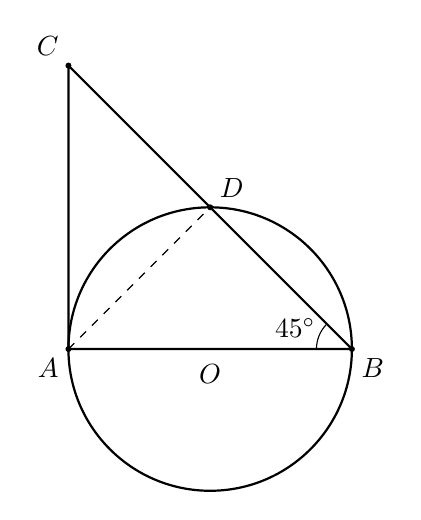
\begin{tikzpicture}[scale=0.9]
  \draw[thick] (0,0) circle (2);
  \coordinate (A) at (-2,0);
  \coordinate (B) at (2,0);
  \coordinate (C) at (-2,4);
  \coordinate (D) at (0,2);
  \draw[thick] (A)--(C)--(B)--cycle;
  \draw[dashed] (A)--(D);
  \fill (A) circle (1.2pt) node[below left] {$A$};
  \fill (B) circle (1.2pt) node[below right] {$B$};
  \fill (C) circle (1.2pt) node[above left] {$C$};
  \fill (D) circle (1.2pt) node[above right] {$D$};
  \node at (0,-0.35) {$O$};
  \draw ([shift={(180:0.5)}]B) arc[start angle=180, end angle=135, radius=0.5];
  \node at (1.2,0.3) {$45^\circ$};
\end{tikzpicture}
\end{center}
\nopagebreak[4]
\Needspace{0.4\textheight}
\end{question}
\begin{question}
\gkti{3}已知长方体 $ABCD\text{-}A'B'C'D'$ 的对角线 $AC'$ 与 $A'C$ 的夹角 $\angle AOC=120^\circ$，底面边长 $AB=4\,\mathrm{cm}$，$BC=3\,\mathrm{cm}$。求此长方体的体积。

\begin{gktip}
\textbf{源注}：原卷印作“$\angle AoC=120^\circ$”“$AB=4Cm$”（字母大小写排印不一致），本库按规范记法转录。
原源 PDF 第 1 页附有长方体及体对角线夹角示意图；LaTeX 版按源图重绘。
\end{gktip}
\nopagebreak[4]
\begin{center}% 1977 年青海卷第三题：长方体 ABCD-A'B'C'D'（顶面 A'B'C'D'），底面 ABCD（A 前左、B 前右、
% C 后右、D 后左），体对角线 AC' 与 A'C 交于体心 O，∠AOC=120°，辅助线底面对角线 AC（虚线）
%（按源卷第 1 页布局）
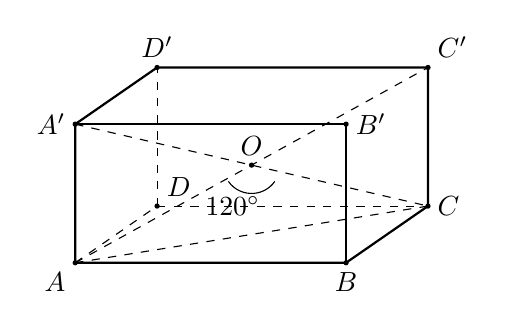
\begin{tikzpicture}[scale=0.8]
  \coordinate (A) at (0,0);
  \coordinate (B) at (4.3,0);
  \coordinate (C) at (5.6,0.9);
  \coordinate (D) at (1.3,0.9);
  \coordinate (A1) at (0,2.2);
  \coordinate (B1) at (4.3,2.2);
  \coordinate (C1) at (5.6,3.1);
  \coordinate (D1) at (1.3,3.1);
  \coordinate (O) at (2.8,1.55);
  \draw[thick] (A)--(B)--(C)--(C1)--(D1)--(A1)--cycle;
  \draw[thick] (A)--(A1);
  \draw[thick] (B)--(B1);
  \draw[thick] (A1)--(B1);
  \draw[dashed] (A)--(D);
  \draw[dashed] (D)--(C);
  \draw[dashed] (D)--(D1);
  \draw[dashed] (A)--(C);
  \draw[dashed] (A)--(C1);
  \draw[dashed] (A1)--(C);
  \fill (A) circle (1.2pt) node[below left] {$A$};
  \fill (B) circle (1.2pt) node[below] {$B$};
  \fill (C) circle (1.2pt) node[right] {$C$};
  \fill (D) circle (1.2pt) node[above right] {$D$};
  \fill (A1) circle (1.2pt) node[left] {$A'$};
  \fill (B1) circle (1.2pt) node[right] {$B'$};
  \fill (C1) circle (1.2pt) node[above right] {$C'$};
  \fill (D1) circle (1.2pt) node[above] {$D'$};
  \fill (O) circle (1.2pt) node[above] {$O$};
  \draw ([shift={(215:0.45)}]O) arc[start angle=215, end angle=325, radius=0.45];
  \node at (2.5,0.9) {$120^\circ$};
\end{tikzpicture}
\end{center}
\nopagebreak[4]
\end{question}
\begin{question}
\gkti{4}求下列函数的定义域：

（1） $y=\dfrac{7x}{x+1}$

（2） $y=\dfrac{1}{\sqrt{2-x}}$

\begin{gktip}
\textbf{题号说明}：原卷两个子项编号为“1．”“2．”，本库按小问格式重排为（1）（2），未增删内容。
\end{gktip}

\end{question}
\begin{question}
\gkti{5}化简：

\begin{gktip}
\textbf{源注}：四次根号内 $b$ 的指数在扫描件中不易分辨，按 600dpi 局部放大目视为 $b^{\frac43}$（无负号），并与源解答中间步骤 $(ab^{-\frac13}\cdot b^{\frac13})^{\frac12}$ 及化简结果 $3a$ 交叉一致。
\end{gktip}

\nopagebreak[4]
\[
\left(27a^{\frac52}\sqrt{ab^{-\frac13}\sqrt[4]{b^{\frac43}}}\right)^{\frac13}\qquad(b\ne0).
\]

\end{question}
\begin{question}
\gkti{6}计算：$\lg14-2\lg\dfrac73+\lg7-\lg18$

\end{question}
\begin{question}
\gkti{7}求 $\sin435^\circ$ 的值。

\end{question}
\begin{question}
\gkti{8}当锐角 $\theta$ 为何值时，方程

\nopagebreak[4]
\[
(3\sin\theta)x^2-(4\cos\theta)x+2=0
\]

有两个相等的实数根？并求出这个方程的实数根。

\end{question}
\begin{question}
\gkti{9}求经过抛物线 $y^2=-2x$ 的焦点，且与直线 $2x-y-1=0$ 垂直的直线方程。

\end{question}
\begin{question}
\gkti{10}今年，我省香日德农场春小麦亩产达 1765.5 斤，创全国春小麦亩产新记录，在大治之年作出了贡献。我省在 1971 年开始出现亩产 1000 斤的高产田。从 1971 年的高产量 1000 斤到今年的创记录产量 1765.5 斤，平均每年的增长率是多少？

（已知 $\lg1.766=0.2470$，已知由 $\lg A=0.0412$ 得 $A=1.100$）

\Needspace{5\baselineskip}
\textbf{参考题 1．} 若齐次线性方程组

\nopagebreak[4]
\[
\begin{cases}
x+ay+a^2z=0\\
ax+a^2y+z=0\\
a^2x+y+az=0
\end{cases}
\]

有非零解，那末 $a$ 应为何值？

\textbf{参考题 2．} 试求由曲线 $y=2\cos x$ 之一半被与 $y=0$ 围成的面积绕 $Ox$ 轴旋转所产生的立体的体积。

\end{question}